\tikzstyle{startstop} = [rectangle, rounded corners, minimum width=3cm, minimum height=1cm,text centered, draw=black, fill=red!30]
\tikzstyle{io} = [trapezium, trapezium left angle=70, trapezium right angle=110, minimum width=3cm, minimum height=1cm, text centered, draw=black, fill=blue!30]
\tikzstyle{process} = [rectangle, minimum width=3cm, minimum height=1cm, text centered, draw=black, fill=orange!30]
\tikzstyle{decision} = [diamond, minimum width=3cm, minimum height=1cm, text centered, draw=black, fill=green!30]
\usetikzlibrary{shapes.geometric}
\tikzstyle{database} = [cylinder, minimum width=3cm, minimum height=1cm, text centered, draw=black, fill=yellow!30, shape border rotate=90, aspect=0.25]

\chapter{Atomic Pair Distribution Function: \\Theory and Computation}
\section{Theory}
To properly understand the PDF and its limitations we need to derive its mathematics.
The following derivation has been performed numerous times but most recently and completely by Farrow and Billinge, it is reproduced here for clarity and completeness.
\subsection{Derivation}
Consider a wave incident on a volume of variable density...
\subsection{Analytical Gradients}
Many optimization algorithms and simulations methodologies, including HMC, require not only the potential energy of a given configuration but also the forces acting on that configuration.
These forces are described by the gradient of potential energy of the system.

\section{Computation}
Simply deriving the equations for the PDF is not enough.
The many body nature of the PDF equation make analytical solution of the structure from the PDF impossible.
Thus, the PDF must be computed from a structural candidates and compared against experimental results to evaluate the relability of the model.

\subsection{HPC and GPUs}
To properly solve the structure of materials the PDF will need to be computed many times and checked against experimental results.
This requires computation of the PDF, potentialy over many atoms.
Calculating these PDFs requires a fast, highly parallized, computational framework.
\subsubsection{GPUs and Parallelization}
Computing the PDF is an embarrassingly parallel problem.
The basic procedure is to calculate the reduced structure factor $F(Q)$ for each atom pair and momentum transfer vector, sum over all the atom pairs, and Fourier transform the structure to the PDF.
The first part of this procedure is perfectly parallizable, as each atom pair is seperate from the others.
The summation over all the atomic reduced structure factors can be parallelized via distributed summing.
Lastly the FFT can be parallelized using existing parellel FFT algorithms.

GPUs are particularly well suted to the task of computing PDFs.
GPU chip architecture is designed to perform many task simultaniously by having potentially thousands of cores.

\subsubsection{Map from ij space to k space}
The above equations, although formally correct, are very ineffiecent. $F(Q)$ and its gradient are indexed over all the atoms twice, however there are symmetries that allow us to only compute over the atom pairs esentially mapping from an $n$x$n$ space, $ij$ space, to a $\frac{n(n-1)}{2}$ space, $k$ space.
For $F(Q)$ we apply the following mapping
\begin{figure}[!ht]
\begin{center}
\begin{tikzpicture}
    \node (E) at (0,0) {$E$};
    \node[right=of E] (F) {$E'$};
    \node[right=of F] (Z) {$Z$};
    \node[below=of F] (N) {$B'$};
    \node[below=of E] (M) {$B$};
    \draw[->] (E)--(F) node [midway,above] {$\psi$};
    \draw[->] (F)--(Z) node [midway,above] {$\Sigma$};
    \draw[->] (M)--(N) node [midway,below] {$\psi'$};
    \draw[->] (E)--(M) node [midway,left] {$\phi$};
    \draw[->] (N)--(Z) node [midway,left] {$\Sigma'$};
\end{tikzpicture}
\end{center}
\end{figure}
where $E$ denotes the atomic coordinates in $ij$ space, $E'$ denotes $F(Q)$ before the summation in $ij$ space, $B$ denotes the atomic pairs in $k$ space, $B'$ denotes $F(Q)$ in $k$ space, and $Z$ denotes the final summed $F(Q)$.  For the operators, $\phi$ denotes the mapping from $ij$ space to $k$ space $k = j + i * \frac{i - 1}{2}$, $\psi$ and $\psi'$ denote the $F(Q)$ operation in $ij$ and $k$ space, respectivly. $\Sigma$ denotes the sum over all the atoms.  

To properly define $\Sigma'$ we must establish whether $F(Q)$ is an even function.  
We can accomplish this by examining each of the portions of $F(Q)$, $\alpha, \beta ,\uptau, \Omega$.
$\Omega$ is even, since $r_{ij}$ is the interatomic distance, which is the same despite a flip of indicies, $Q$ does not depend on the atomic indicies, and since $Qr_{ij}$ is even so is $\sin{Qr_{ij}}$.  Thus, $\Omega$ is even.  Providing similar analysis to $\uptau$ we can see that while $\vec{u}_{ij}$ is odd, so is the unit displacement vector between the two atoms, thus the two odds cancel out.
Intuitivly this makes sense, since the $F(Q)$ equation is fundamentally interested in the interatomic distances which is even.  Thus, switching atom indicies does not change $F(Q)$.
Due to the even nature of the $F(Q)$ operator the $\Sigma'$ operator sums over all the atom pairs, and multiplies by two to reflect the double counting of the $\Sigma$ operator.

For the gradient a similar mapping is used:
\begin{figure}[h!]
\begin{center}
  \begin{tikzpicture}
    \node (E) at (0,0) {$E$};
    \node[right=of E] (F) {$E'$};
    \node[right=of F] (Z) {$Z$};
    \node[below=of F] (N) {$B'$};
    \node[below=of E] (M) {$B$};
    \draw[->] (E)--(F) node [midway,above] {$\psi$};
    \draw[->] (F)--(Z) node [midway,above] {$\Sigma$};
    \draw[->] (M)--(N) node [midway,below] {$\psi'$};
    \draw[->] (E)--(M) node [midway,left] {$\phi$};
    \draw[->] (N)--(Z) node [midway,left] {$\tilde{\phi}\Sigma$};
\end{tikzpicture}
\end{center}
\end{figure}

In this mapping, however, we use the $\tilde{\phi}\Sigma$ operator.  This operator simultaniously performs a reverse mapping from $k$ to $ij$ space, and a summation with the correct symmetry.  In this case the $\psi$ and $\psi'$ operators, which denote the $\grad{F(Q)}$ operator in $ij$ and $k$ space, are antisymmetric.  Intuitivly this makes sense as an extension of Newton's Second Law, since each particle's interation is felt oppositely by its partner.
\subsubsection{Periodic Boundary Conditions}
Periodic boundary conditions can be helpful when simulating extended solids or large nanoparticles. In this case all the non-crystallinity is contained within the simulation box and the box is repeated to create the longer distance peaks observed in the PDF. To perform this we can break up the Debye equation into two main parts, the part that describes the interatomic distances within the simulation box and those between boxes. Neglecting the thermal motion portion:
\begin{equation}
  F(Q) = \frac{1}{N \langle f \rangle^{2}}(\sum_{j\neq i} f_i^{*}(Q)f_j(Q) \frac{\sin(Qr_{ij})}{r_{ij}} + \sum_{i,j} f_i^{*}(Q)f_j(Q) \frac{\sin(QR_{ij})}{R_{ij}})
\end{equation}
where 
\begin{eqnarray}
  R = |\vec{r} + \vec{u}|\\
  \vec{u} = \gamma_1*\vec{a} + \gamma_2*\vec{b} + \gamma_3*\vec{c}
\end{eqnarray}
\section{Experiment}
PDF experiments are generally performed at synchrotron light sources, as only these sources can provide the need flux, energy, and high momentum transfer vectors needed to obtain relyable PDFs.

\section{Data Processing Workflow}
Processing the raw pixel intensities to the PDF is very important as we are extracting most of our interesting information out of very high $Q$ data.
This data relies on good statistics and sound background subtraction.
Talk about papers from Billinge Group with thin film PDF and dilute NP solutions.
Diagram of the overall data processing workflow.
Discuss the NSLS-II data stack.
\begin{landscape}
\begin{center}
\begin{tikzpicture}[thick,scale=0.6, every node/.style={scale=0.6}]
    \node (img) [startstop] at (0,0) {Image Data};
    \node [database, right=of img] (fs)  {FileStore};
    \node[startstop, below=of img] (imeta) {Image Metadata};
    \node[startstop, below=of imeta] (emeta) {Environmental Metadata};
    \node[startstop, below=of emeta] (bmeta) {Beamline Metadata};
    \node[startstop, below=of bmeta] (smeta) {Sample Metadata};
    \node[database, right=of emeta] (mds) {MetadataStore};
    \node[process, right=of mds] (db) {DataBroker};
    \node[io, right=of db] (lfg) {Load Data};
    \node[io, below=of lfg] (lbg) {Load Background};
    \node[process, right=of lfg] (maskfg) {Mask Data};
    \node[process, right=of lbg] (maskbg) {Mask Background};
    \node[process, right=of maskfg] (ifg) {Azimuthally Integrate Data};
    \node[process, right=of maskbg] (ibg) {Azimuthally Integrate Background};
    \node[process, right=of ifg] (bgsubs) {Subtract Background};

%     \draw[->] (img) -- ++(0,1) -- ++($(fs)+(0,1)$)node[] -- (fs);
%     \draw[->] (F)--(Z) node [midway,above] {$\Sigma$};
%     \draw[->] (M)--(N) node [midway,below] {$\psi'$};
%     \draw[->] (E)--(M) node [midway,left] {$\phi$};
%     \draw[->] (N)--(Z) node [midway,left] {$\tilde{\phi}\Sigma$};
\end{tikzpicture}
\end{center}
\end{landscape}
\subsection{MetadataStore Side Loading}
Design of sidewinder-spec for loading the data into metadatastore.
Most of the design considerations went into the loaders, which are different for each experiment.
\subsection{Automated Image Azimuthal Integration}
Mux data as needed. 
Use pyFAI to get the radial distance array.
Note that to properly mask and integrate the system we need to compute the bin edges for the pixels.
The bin edges change as a function of $Q$, as the angle subtended by a pixel shrinks essentially giving high $Q$ pixels more resolution.

\begin{figure}
  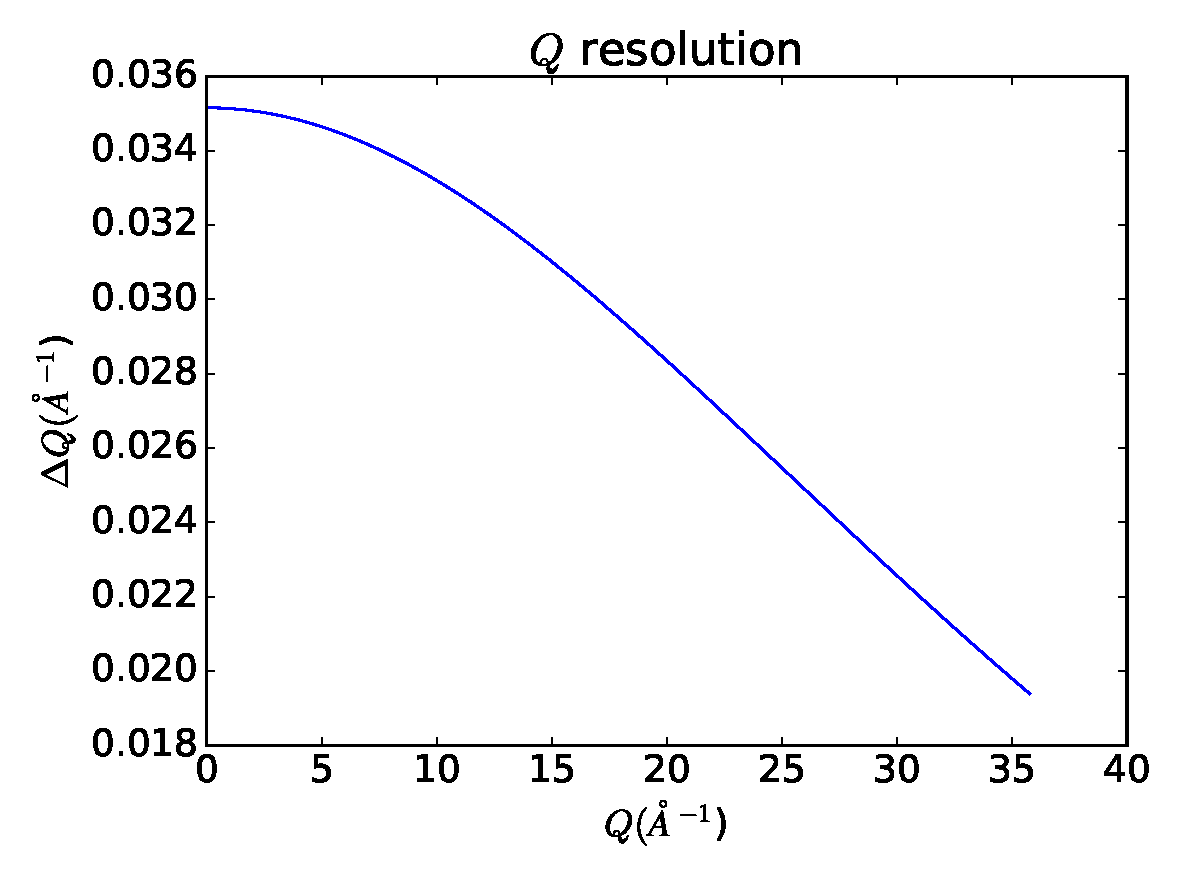
\includegraphics[width=\textwidth]{res}
\caption{$Q$ resolution as a function of $Q$.}
\end{figure}
Mask the image.

\subsubsection{Automated Mask Generation}
Detector masking is an important part of any x-ray scattering workflow as dead/hot pixels, streak errors, and beamstop associated features can be averaged into the data changing the signal and its statistical significance.
While some features, like the beamstop holder, can be easily observed and masked by hand other are much more difficult to observe even on large computer monitors.
Additionally, while dead/hot pixels and streaks are usually static the hot pixels associated with textured or single crystal scattering or cosmic rays are not.
Thus, coming up with an automated method for finding such erroneous pixels is important, especially as high flux diffraction beamlines can generate data very quickly.

While this problem can be quite complex in the most general case, we can use the annular symmetry of the powder scattering pattern to our advantage, by comparing a pixel against pixels in the same ring.
Since non-textured powder scattering should produce the same pixel intensity for a given ring we can mask any pixels which are $x$ standard deviations away from the mean.
This method relies on the aforementioned pixel binning algorithm, as using miss sized bins will cause some pixels which should be in separate rings to be put together, and others which should be in the same ring to be separated.
In that case the masking algorithm will overestimate the number of pixels to be masked due to the additional statistical variation in the sample.

NEED TO INCLUDE FIGURES OF POORLY BINNED PIXELS MASK

ALSO NEED ROTATED BEAMSTOP MASKS

ALSO ALSO NEED TO SHOW THE EFFECT OF CHANGING ALPHA FOR THE MASKING

ALSO ALSO ALSO SHOW SOME MASKS OF REAL DATA, INCLUDING DATA WITH SINGLE CRYSTAL/TEXTURE
 

\foreach \n in {10, 30, 50, 90}{
\begin{figure}
  \foreach \m in {raw, masked, missed}{
    \includegraphics[width=.3\textwidth]{\m_\n}
    }
  \caption{Generated beamstop masks for a beamstop holder with $\n\%$ transmittance. From left to right: the raw image, the masked image, and the missed pixels}
\end{figure}
}

\begin{figure}
\foreach \n in {100, 300, 500, 1000}{
  \foreach \m in {masked}{
    \includegraphics[width=.49\textwidth]{dead_pixel_\m_\n}
    }}
\caption{Generated dead/hot pixel masks for a detector. From top left clockwise: 100, 300, 500, and 1000 dead/hot pixels.}
\end{figure}

Note that we do miss some pixels when the number of dead pixels grows very large.
However, most detectors do not have that many dead pixels.
We can run into these kinds of situations when running samples with some single crystal or textured components. 
However, when this is the case the contrast between the affected pixels and the desired signal is very large enabling easier masking.

We then mask data points 
Additionally the standard deviation threshold can be a function of the pixel distance from the center, allowing the mask generator to be more forgiving at certain points and stricter at others.
This is particularly helpful as the small number of pixels near the point of incidence combined with the very sharp peaks causes some pixels to be improperly masked.
Similarly it is important to remove dead pixels at the edge of the detector as these have an outsized effect on the integration as the pixel intensity is low to begin with.
In practice this results in the removal of almost all dead pixels and potentially the beamstop holder.
Removal of the holder depends on its individual properties, since a holder which is more x-ray opaque will cause a larger shift in the pixel intensity distribution.
The method was benchmarked on synthetic data, with both hot and cold pixels added.
Additional benchmarking was performed with synthetic beamstop holders of various x-ray transmittance.
Anomalous corner masking most likely due to the small number of pixels out at the corners.
